\documentclass[a4paper]{article}

\setlength{\oddsidemargin}{-1in}
\addtolength{\oddsidemargin}{0.05 \paperwidth}
\setlength{\evensidemargin}{-1in}
\addtolength{\evensidemargin}{0.05 \paperwidth}
\setlength{\textwidth}{0.9 \paperwidth}

\setlength{\topmargin}{-0.75in}
\addtolength{\topmargin}{0.05 \paperheight}
\setlength{\textheight}{\paperheight}
\setlength{\headheight}{0in}
\setlength{\headsep}{0in}
\setlength{\footskip}{0in}
	
\usepackage[T1]{fontenc}
\usepackage[utf8]{inputenc}
\usepackage[german]{babel}

\usepackage[default,scale=1.7]{opensans}
\usepackage[scaled=1.6]{beramono}
\linespread{1.9}

\usepackage{url}
\usepackage{graphicx}

\usepackage{grid-system}

\usepackage{color}
\definecolor{freifunkpink}{RGB}{215,0,73}
\definecolor{freifunkyellow}{RGB}{255,191,0}
\definecolor{lightgrey}{RGB}{220,220,220}

\usepackage{enumitem}
\setlist[itemize]{leftmargin=*}

\begin{document}
\thispagestyle{empty}
 
\begin{center}
\Huge \textit{\textbf{\textcolor{freifunkpink}{Freifunk Darmstadt}}} \\
\vspace{0.6cm}
\large ist eine lokale Initiative mit dem Ziel \\
\large ein WLAN-Netzwerk über Darmstadt aufzuspannen \\
\large und freien Internetzugang anzubieten.
\normalsize

\vspace{1.5cm}

\hspace*{-0.05 \paperwidth}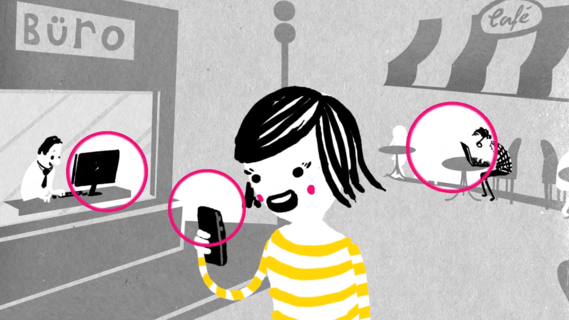
\includegraphics[width=\paperwidth]{verbindet}
\end{center}

\vspace{0.7cm}

\begin{Row}
    \begin{Cell}{1}
    \textbf{How does it work?} \\
Freifunk-Netze sind Selbstmach-Netze. Auch du kannst mit einfachen Mitteln dazu
 beitragen, indem du einen Teil deiner Netzwerkressourcen anderen zur Verfügung
 stellst. Wenn viele mitmachen, entsteht ein flächendeckendes freies WLAN-Netzw
erk in Darmstadt.
    \end{Cell}
    \begin{Cell}{1}    
    \textbf{Advantages for commercial spaces:} \vspace*{-0.18cm}
	\begin{itemize}
	   \item[\textcolor{freifunkpink}{\Large$\bullet$}] no risks \vspace*{-0.3cm}
	   \item[\textcolor{freifunkpink}{\Large$\bullet$}] no user registration required \vspace*{-0.3cm}
	   \item[\textcolor{freifunkpink}{\Large$\bullet$}] nicht kommerziell \vspace*{-0.3cm}
	   \item[\textcolor{freifunkpink}{\Large$\bullet$}] no running costs \vspace*{-0.3cm}
	   \item[\textcolor{freifunkpink}{\Large$\bullet$}] free internet is cool\vspace*{-0.3cm}
	   \item[\textcolor{freifunkpink}{\Large$\bullet$}] our sticker is cool\vspace*{-0.3cm}
	   \item[\textcolor{freifunkpink}{\Large$\bullet$}] we can provide support
	\end{itemize}
    \end{Cell}
\end{Row}
\newpage

\thispagestyle{empty}

\begin{Row}[cellsep=0.75cm]
    \begin{Cell}{1}
    \textbf{Was kann man damit tun?} \\
    Durch Freifunk werden z.B. lizenzfreies Community-Radio, die Übertragung lokaler Events, Telefonieren, Chatten, der Austausch öffentlicher Dateien und die gemeinsame Nutzung eines Internetanschlusses möglich. -> local homepage in the city, no need to pay for servers, for example
    \end{Cell} 
\begin{Cell}{1}
    \textbf{Kein Risiko für dich} \\
Freifunk Darmstadt hilft dir dabei, ein passendes Gerät zu finden und einzurichten. Dieser sogenannte Freifunkknoten leitet den Datenverkehr anonymisiert ins Internet. Dadurch kann der Datenverkehr anderer nicht auf deine Verbindung zurückgeführt werden.
\end{Cell}
\end{Row}

\vspace{1.3cm}
\begin{Row}
    \begin{Cell}{1}
	If you have questions and/or want to participate, contact us at info@freifunk-darmstadt.de
	\end{Cell}
\end{Row}
\vspace{0.5cm}
\begin{center}
	\large Mehr Infos: \url{darmstadt.freifunk.net}
\end{center}
\begin{center}
\vspace{-0.5cm}
\hspace*{-0.05 \paperwidth}\includegraphics[width=\paperwidth]{DA-logo_trans}

\vspace{-2.7cm}
\large \textcolor{lightgrey}{Twitter: \textit{@freifunkda}}
\end{center}
\end{document}
